\documentclass{tufte-book}

\hypersetup{colorlinks}% uncomment this line if you prefer colored hyperlinks (e.g., for onscreen viewing)

% Book metadata
\title{Introduction to Experimental Physics}
\author[Physics 229]{Phys 229}
\publisher{Andrew MacRae}

%%
% If they're installed, use Bergamo and Chantilly from www.fontsite.com.
% They're clones of Bembo and Gill Sans, respectively.
\IfFileExists{bergamo.sty}{\usepackage[osf]{bergamo}}{}% Bembo
\IfFileExists{chantill.sty}{\usepackage{chantill}}{}% Gill Sans

%\usepackage{microtype}

\usepackage{amsmath}

% Just some sample text
\usepackage{lipsum}

% Probably don't need thius
\newcommand{\doccls}[1]{\texttt{#1}}% document class name

%%
% For nicely typeset tabular material
\usepackage{booktabs}


% For graphics / images
\usepackage{graphicx}
\setkeys{Gin}{width=\linewidth,totalheight=\textheight,keepaspectratio}
\graphicspath{{Images/}}

% The fancyvrb package lets us customize the formatting of verbatim
% environments.  We use a slightly smaller font.
\usepackage{fancyvrb}
\fvset{fontsize=\normalsize}

%%
% Prints argument within hanging parentheses (i.e., parentheses that take
% up no horizontal space).  Useful in tabular environments.
\newcommand{\hangp}[1]{\makebox[0pt][r]{(}#1\makebox[0pt][l]{)}}

%%
% Prints an asterisk that takes up no horizontal space.
% Useful in tabular environments.
\newcommand{\hangstar}{\makebox[0pt][l]{*}}

%%
% Prints a trailing space in a smart way.
\usepackage{xspace}
% To give mad credit
\newcommand{\TL}{Tufte-\LaTeX\xspace}


% Prints the month name (e.g., January) and the year (e.g., 2008)
\newcommand{\monthyear}{%
  \ifcase\month\or January\or February\or March\or April\or May\or June\or
  July\or August\or September\or October\or November\or
  December\fi\space\number\year
}

% Prints an epigraph and speaker in sans serif, all-caps type.
\newcommand{\openepigraph}[2]{%
  %\sffamily\fontsize{14}{16}\selectfont
  \begin{fullwidth}
  \sffamily\large
  \begin{doublespace}
  \noindent\allcaps{#1}\\% epigraph
  \noindent\allcaps{#2}% author
  \end{doublespace}
  \end{fullwidth}
}

% CUstom Colors
\definecolor{greenExample}{RGB}{61,170,61}
\definecolor{greenExampleBack}{RGB}{216,233,213}


\usepackage[many]{tcolorbox}
% Define example environment
\newtcolorbox[auto counter, number within=chapter]{myexample}[2][]
{%
  breakable,
  enhanced,
  colback=white,
  colbacktitle=white,
  arc=0pt,
  leftrule=1pt,
  left skip = 6pt,
  rightrule=0pt,
  toprule=0pt,
  bottomrule=0pt,
  titlerule=0pt,
  colframe=greenExampleBack,
  fonttitle=\normalcolor,
  overlay = 
  {
    \node
    [
      outer sep=0pt,
      anchor=east,
      text width=2.5cm,
      minimum height=4ex,
      fill=greenExampleBack,
      font=\color{greenExample}\sffamily\scshape
    ] 
    at (title.west) {example~\thetcbcounter};
  },
  title=#2,
  #1
}
\newcommand\Solution{\par\textbf{\textsf{Solution}}\par\medskip}

% Generates the index
\usepackage{makeidx}
\makeindex

\begin{document}
% Front matter
\setcounter{chapter}{1}
\frontmatter

% r.1 blank page
%\blankpage

% v.2 epigraphs
\newpage\thispagestyle{empty}
\openepigraph{%
In theory, there is no difference between theory and practice. But, in practice, there is.
}{Yogi Berra%, {\itshape Design, Form, and Chaos}
}
\vfill
\openepigraph{%
A designer knows that he has achieved perfection 
not when there is nothing left to add, 
but when there is nothing left to take away.
}{Antoine de Saint-Exup\'{e}ry}


% r.3 full title page
\maketitle

% r.9 introduction
\cleardoublepage
\chapter*{Introduction}

Wha?
and the use of the \doccls{tufte-book} and \doccls{tufte-handout} document classes.


%%
% Start the main matter (normal chapters)
\mainmatter


\chapter{Fundamental Quantities of Electronics}
\label{ch:fundamentals}

\section{What is Electronics?}

\newthought{Take an electronic device} which can be as simple (a flashlight) or as complicated (a smartphone) as you like. Fundamentally, these devices function by using electric and magnetic fields to push around charged particles which wiggle and bump into one another in just the right way to work as they do. All of this behaviour can be precisely calculated using Maxwell's equations (which you will see very soon in your physics career if you haven't already). Although that is what is truly what is going on ``behind the scenes'', it is a terribly impractical and unpleasant way of thinking about a flashlight. The goal of electronics is to encapsulate all of this complexity into much simpler abstract models. In other words, we want to simplify the flashlight into a cartoon drawing, the flashlight in the same way that we simplify the motor, suspension, and materials of a car in first year physics (figure \ref{fig:abstraction}).

\begin{figure}
  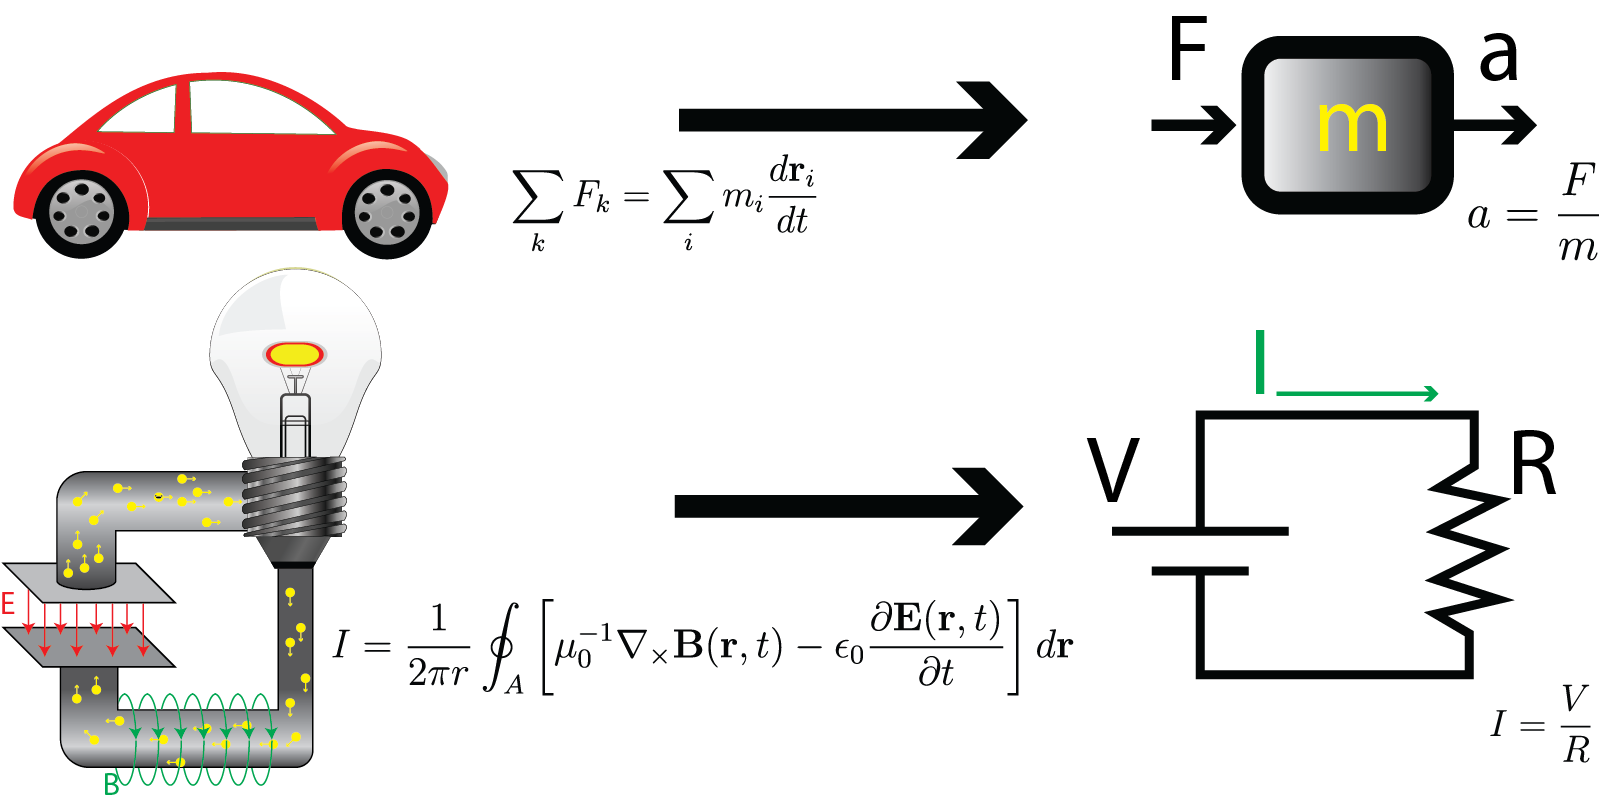
\includegraphics{abstraction}
%  \checkparity This is an \pageparity\ page.%
  \caption{Just as you can calculate the acceleration of a car with mass $m$ and \textit{net} force $F$ without knowing the internal details, the electronics formalism allows you calculate the current through a lightbulb given its resistance and voltage, without bothering about the particular construction or electromagnetic fields.}
  \label{fig:abstraction}
  %\zsavepos{pos:textfig}
  \setfloatalignment{b}
\end{figure}


\section{Fundamental Electronic Quantities: Charge, current, and Voltage}
\subsection{Charge} Charge is a fundamental property of a body and can be negative, positive, or zero (neutral). The S.I. units of charge is the Coulomb [C]. In nature charge is carried by (positive) protons and (negative) electrons\footnote{particle physicists will have a slightly longer list.} having equal magnitude but opposite sign, and the net charge of a body is entirely due to an imbalance between protons and electrons. The charge of an electron is a fundamental constant given approximately by $q_e \approx 1.602\times10^{-19}$ C. 

\subsection{Current} Electronics is concerned with the transport of charge by means of electric and magnetic fields. The force on a charge $q$ due to an electric field $\textbf{E}$ is given by: $\textbf{F} = q\textbf{E}$.\footnote{There is an additional force on a moving charge due to a magnetic field. The more general expression is given by the Lorentz force: $\textbf{F} = q\textbf{E} + q\textbf{v}_\times\textbf{B}$.} The \textit{current} passing through an area $A$ is defined as the amount of charge passing through this area per unit time (see fig. \ref{fig:curr}):

\begin{equation}\label{eq:defn_current_words}
\text{current} = \frac{\text{net charge though surface}}{\text{unit time}}
\end{equation}

\noindent The SI unit of current is the ampere which is a Coulomb per second: 1A = 1C/s.

\begin{marginfigure}%
  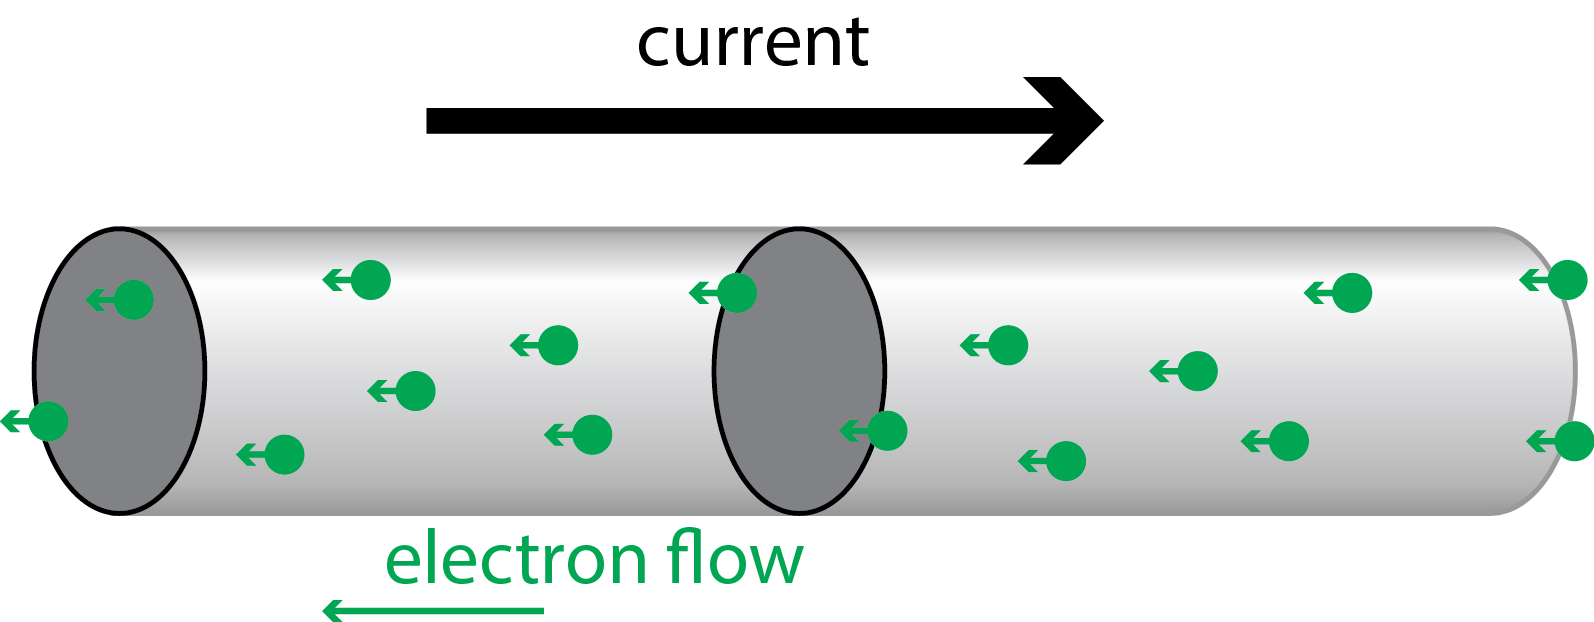
\includegraphics[width=\linewidth]{currentflow}
  \caption{Current in a wire is the amount of charge passing a given cross section of the wire per unit time. Note that due to the negative charge of the electron, the direction of the current is opposite that of the electrons' velocity.}
  \label{fig:curr}
\end{marginfigure}

In electronics we deal with current sufficiently large that we can safely ignore the discrete nature of electrons and treat charge as continuous ``electric fluid'' that can flow (see example \ref{ex:current_is_cts}). This allows us to define the current more rigorously as:
\begin{equation}\label{eq:defn_current}
I \equiv \frac{dq}{dt}
\end{equation}


\begin{myexample}[label = ex:current_is_cts]{The smallest values of current in practice are on the nA ($10^{-9}$A) level. How many electrons pass through a wire per second for 1~nA of Current?}
\Solution
1 nA corresponds to $1\times10^{-9}~\frac{C}{s}$. An electron on the other hand carries approximately $\vert q_e\vert = 1.6\times10^{-19}$~C of charge. A wire conducting 1~nA of current thus sees:
$$
\left(1\times10^{-9}~\frac{C}{s}\right)\times\left(\frac{1~e}{1.6\times10^{-19}C}\right) = 6.25\times10^9\frac{e}{s} 
$$
pass through. Thus, even then, this corresponds to a flow of about 6 billion electrons per second.
\end{myexample}

Note that current is defined to be in the direction of positive charge - the in a typical situation where negatively charged electrons carry the charge, the current is opposite the direction of the charges! 

Typical values for current in electronic devices are on the order of milliamps (1mA = $10^{-3}$A) tens of mA is already dangerous to humans and 1A can easily start fires. We will discuss the heat generated by current shortly. 

\subsection{Voltage/Potential Difference}: You may recall from earlier courses that there is a quantity known as an electric potential $\phi$ which has units  of volts, or equivalently, Newtons per Coulomb (1V = 1N/C). The potential due to a point charge $q$ at distance $r$ is given as $\phi = \frac{1}{4\pi\epsilon_0}\frac{q}{r}$ and the potential due to arbitrary charge distributions can be easily stated\footnote{Though not always easily calculated}. The utility of $\phi$ is that once given it allows you to easily determine the electrical potential energy:

\begin{equation}\label{eq:elec_pot}
E = q\phi
\end{equation}

Being an energy, the unit of electrical potential energy is the Joule, but a convenient and commonly equivalent unit is the electron volt (eV). Self-explanatorily, this is the energy acquired by an electron when it's electrical potential has changed by one volt. From the value of the electron charge and equation \ref{eq:elec_pot}, we see that:

\begin{equation}\label{eq:defn_eV}
1 \text{ eV} = 1.602\times10^{-19}\text{ J}
\end{equation}

\begin{myexample}[label = ex:energy_lhc]{The Energy Scale of the LHC}
Upon re-opening in 2015, the Large Hadron Collider (LHC) accelerated a beam of protons, each having an energy of nearly 6 TeV ($6\times10^{12}$ eV).

Let's Compare this to the energy of a grain of sand at a height of 1~m. The gravitational potential energy is given by $E = mgh$ Plugging in numbers, this is about 0.01~J or about $6\times10^{16}$ eV or roughly 10000 times that of the LHC!

While this may not seem terribly efficient, recall that there are roughly $10^{24}$ protons in a grain of sand, so the energy \textit{per particle} in the LHC is higher by a factor of roughly $10^{20}$.

\end{myexample}


Like gravitational potential, there is no absolute scale -- only differences in potential are physically meaningful. This leads us to the definition of \textit{voltage} or, as you may now see why, \textit{potential difference}. Referring to figure \ref{fig:volt_ref}a, the voltage between two points $A$ and $B$ is:

\begin{equation}
  \boxed{V = \phi(B)-\phi(A)}
\end{equation}

\begin{figure}
\caption{(a) The voltage between two points is defined as the difference in electric potential. (b) Circuit symbols for a voltage source and electrical ground. (c) A complete circuit connected through ground.}
\label{fig:volt_ref}
\begin{center}
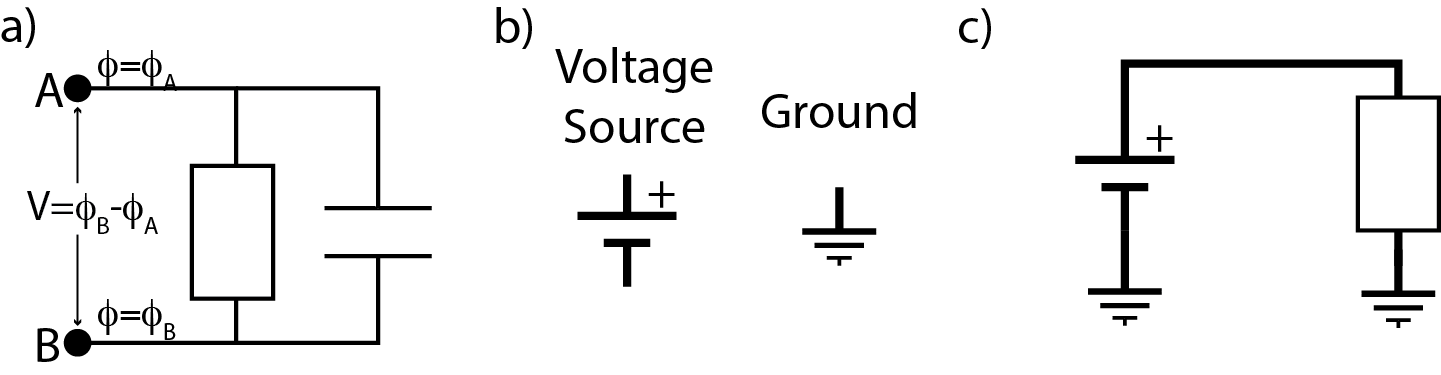
\includegraphics[width=\textwidth]{volt_ref}
\end{center}
\end{figure}

An ideal voltage source is something (anything) which can maintain a fixed electric potential between two points. What is meant by a non-ideal source will be discussed next lecture. Note that we don't care how it is made - it could be a battery, solar generator, or bench-top power supply. We draw an ideal voltage source, regardless of its construction as in figure \ref{fig:volt_ref}b. We thus arrive at our first layer of abstraction, and will continue to replace complicated devices by little cartoon which simplify design significantly throughout the course.

A key concept is that of electrical ground, often called \textit{ground}, or ``earth''. Since voltages are always defined with respect to a reference voltage, a given point in a circuit is often denoted as the 0V point, against which all other measurements are made. Ground in a circuit is so important that it is given a special symbol (figure \ref{fig:volt_ref}c. 

\begin{figure}
\caption{(a) A ground connection outside some house in Australia (Wikipedia CC licence) (b) All ground points in a circuit are connected.}
\label{fig:ground_ref}
\begin{center}
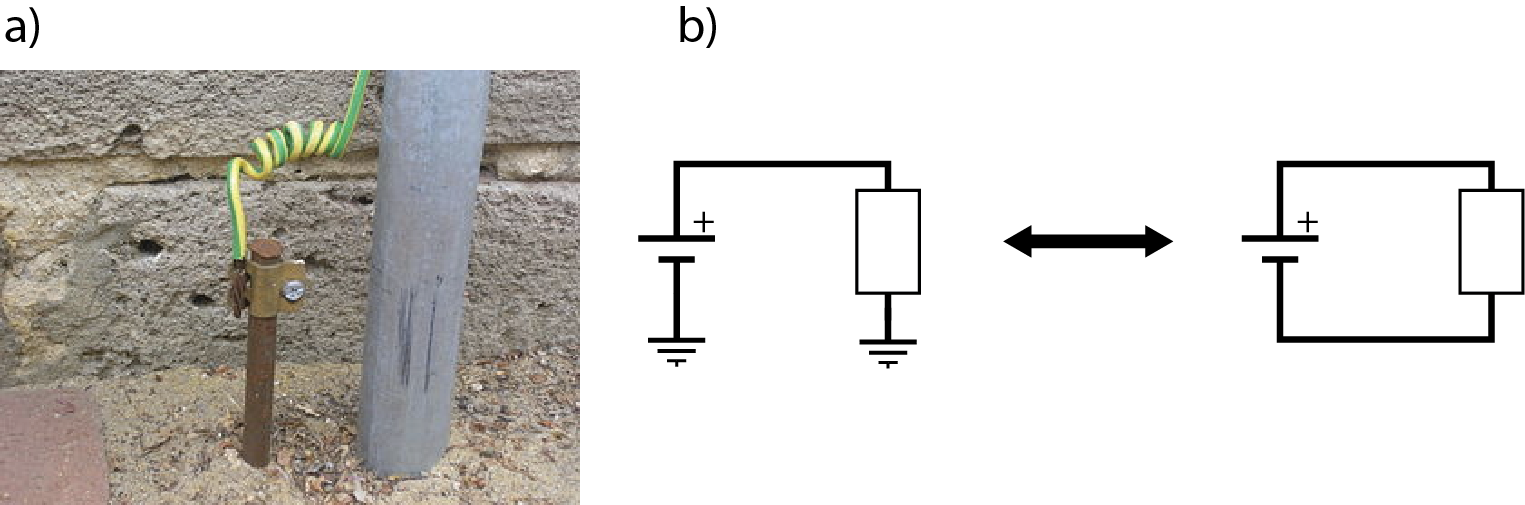
\includegraphics[width=\textwidth]{ground_and_pound}
\end{center}
\end{figure}

The name ground is quite literal -- it is often connected to a large stake driven into the Earth (fig. \ref{fig:ground_ref}a. The reason for this is that the (literal) ground provides a very large neutral body which whose potential will not change even when large amount of current are flowing into it. This would not be the case for a small metal plate which would develop a large charge imbalance and thus acquire a positive voltage. It is important to note that although not explicitly drawn, all ground connections are connected as if by a physical wire. 

The potential of the dirt outside your window need not be the reference voltage for $V=0$. Devices powered by a battery are clearly not connected physically to earth ground. Such devices are said to be \textit{floating} and the ground is often defined as the negative terminal of the battery. The term floating means that while the voltage \textbf{differences} are well defined along the circuit, their \textbf{absolute value} compared to an external reference are not and thus the ground level of two separate devices may float around with respect to one another. This can cause a significant danger when two floating devices are connected: since they do not have a common value for ground, they high potential differences between the two devices can exist which will damage the device. 

\section{Wires, conductors, and insulators}
Just as masses in a gravitational potential will tend to accelerate to the lower potential, so to will current flow from a higher to a lower potential. To do so however, they charges need a path. As electrons are typically bound to their atoms via the coulomb force, they are typically sitting in their own potential well. This is why current isn't spontaneously flowing from one terminal of a battery to the other despite having a potential difference. Note however that if a sufficiently strong voltage is applied current will flow - even in vacuum. Certain materials however have electronic structure such that an individual electron is not bound to a particular atom and is free to move along an atomic ensemble, as long as it is replaced by another. These materials, known as conductors form the basis of electronic conductors. As long as one conductor maintains good contact with another, current may flow freely between them. The ease by which current flows is parametrized by the \textit{conductance} $\rho$ and has units of Siemens per meter.

At the opposite end of the spectrum are insulators which have electronic structure such that all electrons are tightly bound, giving them a very low conductivity. Insulators are as important as conductors in electronics as they provide the ``walls'' which keep current from flowing everywhere. It turns out that there is a third class of material we will deal with in this course which is somewhere in between a conductor and an insulator. Such a substance is known as a semiconductor. What makes semiconductors useful is that their conductivity can be easily tuned by introducing impurities and can by manipulated by injecting charges in between two different semiconductors. We will examine semiconductors in detail later in the course. Table \ref{tab:conduct} gives an overview of the conductivity of various materials.

\begin{table}[]
\centering
\caption{Electrical properties of various materials}
\label{tab:conduct}
\begin{tabular}{lll}
\hline
Material    & Classification & Conductivity {[}S/m{]} \\ \hline\hline
Copper      & Conductor      &          $5.96\times10^7$             \\
Aluminum        & Conductor      &             $3.50\times10^7$           \\
Hard Rubber        & Insulator      &             $1.0\times10^{-14}$      \\
Quartz        & Insulator      &             $1.30\times10^{-18}$           \\
 Silicon & SemiConductor      &          0.01 -- 1000 [depending on doping]            \\ \hline
\end{tabular}
\end{table}

Wires form the basis of our next idealization/abstraction. Although wire contain a complex lattice of various atomic structure we treat them in our circuit as perfect conductors of electricity which allow us to instant transfer an electric potential from one place in a circuit to another (i.e. lines of equipotential). In a circuit diagram we draw them as lines and in our conceptualization, we think of them as ``electricity pipes'' which current flows though without resistance. 


\section{Resistors and Resistivity}

The conceptualization of current carrying wires as pipes leads to an oft-used and useful analogy in electronics: we can visualize the flow of charge as we would the flow of water through a pipe as sketched in figure \ref{fig:water_analogy}. In this analogy voltage sources are replaced with hydraulic pumps and potential differences are pressure differences and current is fluid flow. The conductivity is given by the pump width. 

\begin{figure}[h]
\caption{In the Hydraulic analogy, voltage sources are pumps, voltage is pressure, and resistance is pipe constriction.}
\label{fig:water_analogy}
\begin{center}
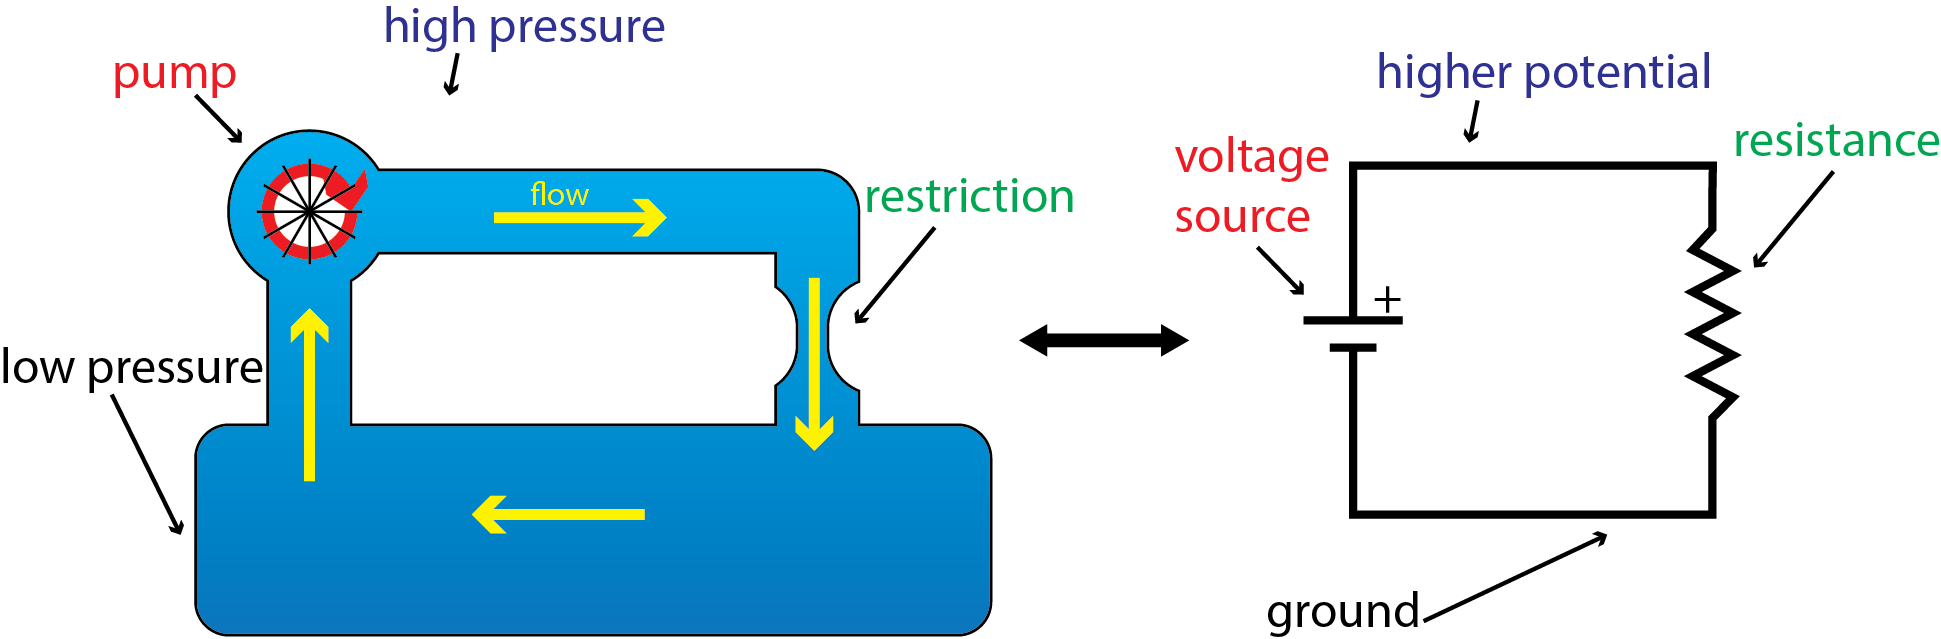
\includegraphics[width=\textwidth]{waterpumpanalogy.png}
\end{center}
\end{figure}

As you may imagine from the above analogy a wide, short wire will have an easier time passing current than  long thin one, which indeed turns out to be the case. The ease with which a given circuit element passes current for a given voltage is known as the resistance, defined as:

\begin{equation}\label{eq:def_res_op}
R \equiv \frac{V}{I}
\end{equation}

It turns out that for a conductor, the resistance can be determined from its geometry and conductivity, or as is most often used, its inverse -- the resistivity:

\begin{equation}\label{eq:def_resistivity}
\rho \equiv \sigma^{-1}
\end{equation}

Specifically, for a wire with resistivity $\rho$, cross sectional area $A$ and length $L$, the resistance is given by:

\begin{equation}\label{eq:def_resistance}
R = \rho\frac{L}{A}
\end{equation}

Consistent with the water analogy the longer the wire, the higher the resistance, but this can be compensated by increasing its area (think of blowing through a long stir stick vs. a giant bubble tea straw -- which is harder?).

For certain circuit elements the ratio in equation \ref{eq:def_res_op} is constant for all voltages. These devices are said to be ``Ohmic'' and obey \textit{Ohm's Law}.

\begin{equation}\label{eq:ohmslaw}
  \boxed{V = IR}
\end{equation}

\noindent  \textcolor{red}{\textbf{WARNING}}: many circuit devices are non-ohmic and do not satisfy Ohm's law. In some texts, Ohmic just means a resistor, and non-Ohmic means anything else. To go further, \textbf{nothing} in nature is truly Ohmic since nothing is truly linear, but for Ohmic materials, the nonlinearity is so small that the point is moot. Whether or not a device is Ohmic can be determined by plotting voltage as a function of current by means of a so-called ``IV curve''. An IV curve for a resistor and for a non-Ohmic device is shown in figure \ref{fig:ohmic}.

\begin{marginfigure}%
  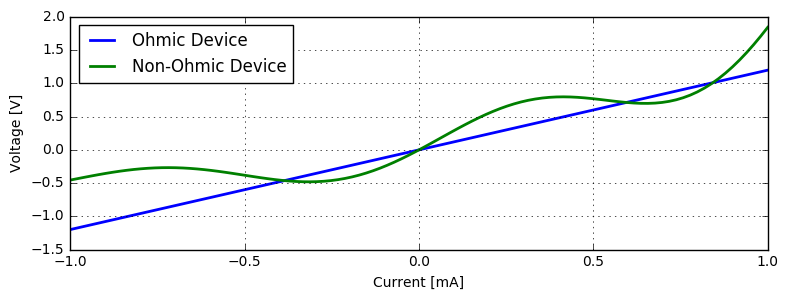
\includegraphics[width=\linewidth]{ohmicnonohmic}
\caption{Many devices are non-ohmic. The ratio of voltage to current is constant for resistors (blue) which obey Ohm's law. Other materials are non-Ohmic and have a non-constant slope (green) }
  \label{fig:ohmic}
\end{marginfigure}


Resistors are constructed by taking a conductor with a given resistivity $\rho$ and very carefully tuning the geometry to create a well defined resistance via equation \ref{eq:def_resistance}. There are several design techniques: wire-wound resistors are made by taking a very thin wire and wrapping it around a coil until a desired length - and thus resistance is achieved. Thin film resistors take an opposite approach and tune the area of a fixed length film via the thickness. In either case the resistors are encases by an insulating material and placed in a compact package. Conducting leads allow the resistor to connect to other circuit elements. Figure \ref{fig:someresistors} displays some of the existing technologies.

\begin{marginfigure}%
  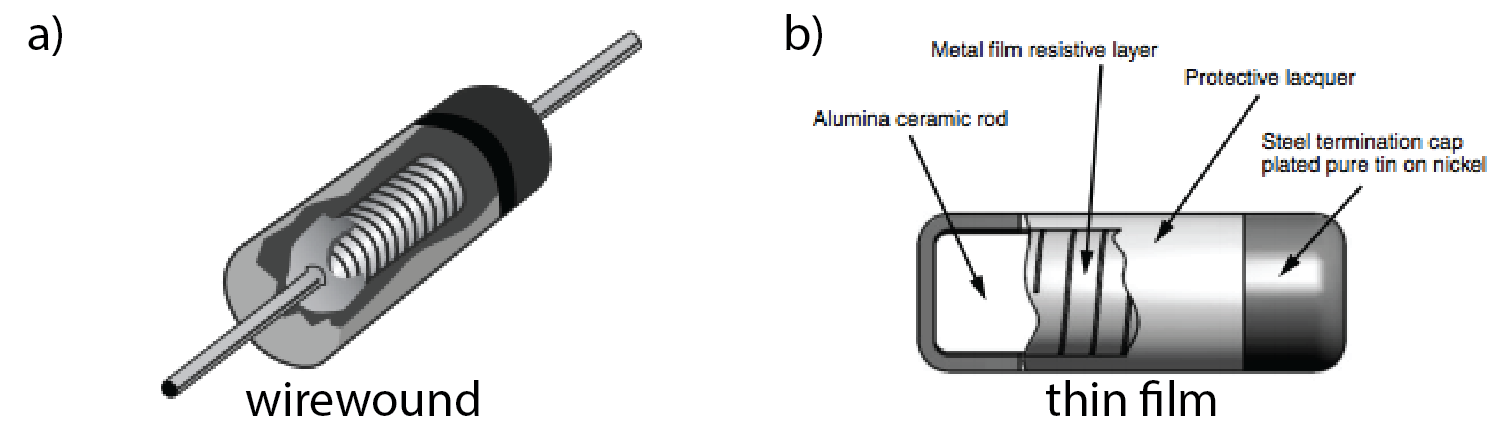
\includegraphics[width=\linewidth]{someresistors}
\caption{Sketch of a wirewound (a) and thin-film (b) resistor. Image from Vishay application note 28771}
  \label{fig:someresistors}
\end{marginfigure}

You may also notice coloured rings on the resistors you use in the lab. This is the resistor colour code that allows you to determine the resistance by cross-referencing with a look-up table. Such a table is included in the manual of Lab 1.  Some gurus may take pride in memorizing the resistor colour code and can tell you that you are holding a 12k$\Omega$ resistor just by looking at it.

There are also variable resistors known as potentiometers which you will become familiar with in the lab. These work by having a moving conducting terminal which can slide along the resistor, continuously changing the length and therefore via eq. \ref{eq:def_resistance}, the resistance.


\subsection{Resistance of Non-Ohmic Devices}
\newthought{Note the} distinction between equations: \ref{eq:def_res_op} and \ref{eq:ohmslaw}. The latter implies that there is a linear relationship between voltage and current, and the ratio is the resistance. Equivalently, when plotted on an IV curve, the slope of the plot is the resistance.

This leads to two generalizations of resistance as either the ratio or the slope:

\begin{subequations}
\begin{align}
    R_{s} = \frac{V}{I}\label{eq:genres1}\\
   R_d = \frac{dV}{dI} \label{eq:genres2}
\end{align}
\end{subequations}

The quantity $R_s$ is known as the ``static resistance'' and $R_d$ is the differential resistance. Note that unlike static resistance which is necessarily positive, the a device can have negative differential resistance, meaning that $R_s$ decreases with increasing current. The regions $-0.7\text{ mA}  < I < -0.3\text{ mA}$ and $0.4\text{ mA}  < I < 0.7\text{ mA}$ in figure \ref{fig:ohmic} display this.

One common example of negative differential resistance is the fluorescent light bulbs which are installed in most office buildings. As more current flows, the bulb becomes more conductive. To circumvent a runaway process in which more and more current is drawn until a catastrophic failure (i.e. explosion) occurs, fluorescent lights are powered by ``ballasts'' that switch the current at high frequencies. In lab 10, you will construct an optical sensor to measure this switching frequency.


\subsection{Electrical Power and Joule Heating}
Ohms law tells us that when current flows through a resistor there is a drop in voltage and therefore a drop in the energy of each charge in the current. Given that energy is conserved, where does this energy go? It turns out that on the microscopic scale, the electrons comprising the current undergo inelastic collisions with the lattice of the material. It is just the likelihood of these elastic collisions which determine the conductivity/resistivity of the material. 

Recall that in an inelastic collision, the particles lose kinetic energy and it this is just the case here. The electrons are accelerated by being in an electric potential until they collide with an ion in the lattice and bounce off, with less kinetic energy than they had before. Since the lattice ions are fixed, all of their motion goes into vibrations and we know this random atomic-lattice vibration as heat. This effect is known as \textit{Joule Heating}.

As the electrons are dumping a given amount of energy per unit time due to the current, this heating is a power having units of Watts (1W = 1J/s). The general expression for the heating due to a current $I$ across a potential difference $V$ is remarkably simple, and is given by:

\begin{equation}\label{eq:joule_gen}
\boxed{P=IV}
\end{equation}

For Ohmic materials, we can use Ohm's law to re-write this solely in terms of voltage and resistance:

\begin{equation}\label{eq:joule_ohm}
P = I^2R = \frac{V^2}{R}
\end{equation}

This is actually how incandescent light bulbs work. They they are formed by a thin wire having a non-ohmic resistance\footnote{The reason that the wire here is non-ohmic is that it heats up considerably which leads to more collisions and thus higher resistance} and the Joule effect causes them to heat up until they glow white-hot. Older lightbulbs are thus simply heaters that get so hot they happen to glow. They are also remarkably inefficient -- only about 2\% of their power is converted into visible light. A modern white-light LED on the other hand can reach nearly 50\%.



\begin{myexample}[label = ex:res_lightbulb]{The resistance of a 60W light bulb}
A 60W light bulb means that at wall-voltage (120V) the filament can safely absorb 60W of heat. What is the current of the light when operating at 60W? What is the static resistance?
\Solution % uncomment for solution style
From equation \ref{eq:joule_gen}, we see that $I = P/V = 60W/120V = 0.5A$. Thus we see that a current of 500 mA is drawn. The (static) resistance is then 
$$
R_s = V/I = 120V/0.5A = 240 \Omega
$$
\end{myexample}



% \noindent\textbf{Pop Quiz}:

% \noindent(a) Does the current increase/remain equal/decrease? 

% \noindent(b) Is the resistance higher/equal/lower? 


\section{Connecting resistors}
A real circuit does not typically contain a single battery pushing current through a single resistor. There is a network of resistors, and other components which we will learn about shortly. When resistors are connected together they simply form a new resistor of a different resistance. Since resistors are two-terminal devices, it turns out that there are only two basic ways that a pair of resistors can be connected:

\begin{figure}[h]
\caption{Sketch of Series and parallel connections}
\label{fig:res_series_parallel}
\begin{center}
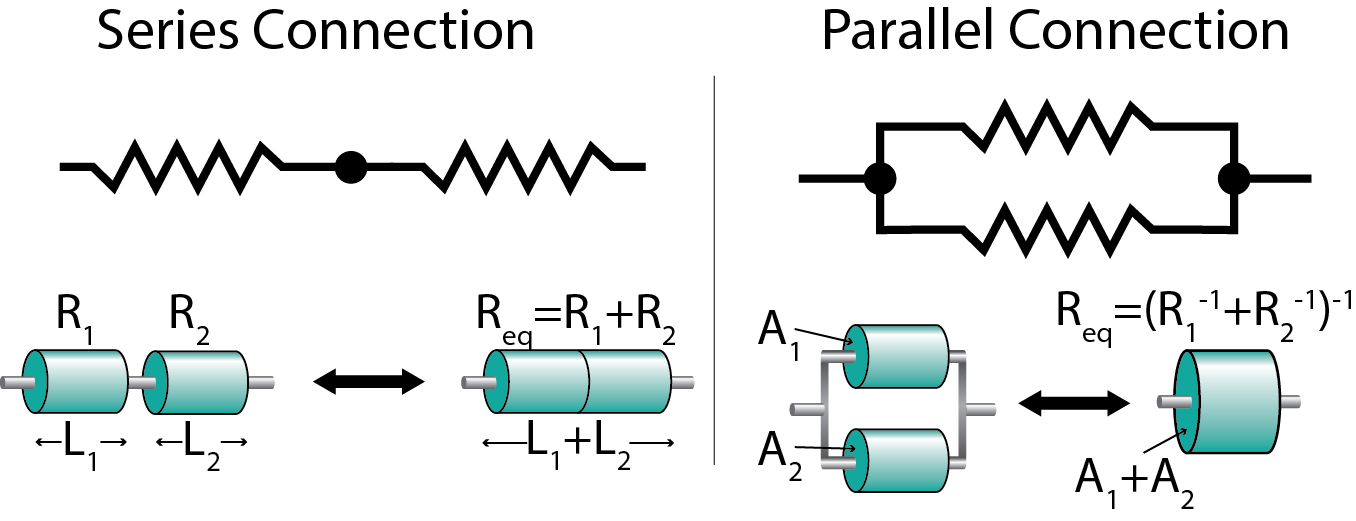
\includegraphics[width=\textwidth]{res_series_parallel.png}
\end{center}
\end{figure}


\subsection{Series connection} In a series connection the resistors are placed end to end and all of the current is forced to flow through both resistors. The voltage drop is split between the two resistors. Referring to figure \ref{fig:res_series_parallel}, we see that this is equivalent to increasing the length of the resistor and thus the resistance increases. To understand this more quantitatively, consider two resistors of equal area $A$ and lengths $L_1$ and $L_2$ such that the resistances are $R_1$ and $R_2$ given equation \ref{eq:def_resistance}. Connecting them in parallel then leads to a new resistor with length $L = L_1 + L_2$ with resistance $R = \rho\frac{L}{A} = \rho\frac{L_1}{A} + \rho\frac{L_2}{A} = R_1 + R_2$.  This is true in general:

\begin{equation}\label{eq:series_res}
\boxed{R_{\text{series}} = R_1+R_2}
\end{equation}

\subsection{Parallel connection} In a parallel connection, the current is split between two resistors but the voltage drop is the same across both since they are connected to a common node. From the figure we see that two resistors in parallel are equivalent to a single resistor with greater area. The resistance of a series connection is thus less than that of its constituent resistors. To get more quantitative again, consider two resistors with equal length $L$ and resistivity $\rho$, but different areas $A_1$ and $A_2$, yielding resistances $R_1$ and $R_2$. The resistance of the parallel connection is given by $R = \rho\frac{L}{A} = \rho\frac{L}{A_1+A_2}$. Therefore we have: $R^{-1} = \frac{A_1+A_2}{\rho L} = \frac{A_1}{\rho L} + \frac{A_2}{\rho L} = R_1^{-1} + R_2^{-1}$. We thus arrive at the equivalent resistance of a parallel resistance:

\begin{equation}\label{eq:series_par}
\boxed{R_{\text{parallel}} = \left(R_1^{-1}+R_2^{-1}\right)^{-1} = \frac{R_1R_2}{R_1+R_2}}
\end{equation}

\textbf{An Important Approximation:} In many cases in practice, a series or parallel combination is completely dominated by one of the two resistors. Consider two resistors: $R_1 = 10\text{ k}\Omega$ and  $R_2 = 50\text{ }\Omega$. The parallel combination of the two gives $R_{\text{series}} = 10$ k$\Omega$ + $50\text{ }\Omega = 10.05\text{ k}\Omega \approx 10\text{ k}\Omega$. On the other hand, the parallel connection gives $ R_{\text{parallel}} = \frac{50\Omega\times10^4\Omega}{10050\Omega} = 49.751\ldots \approx 50\Omega$. 

\noindent Thus if $R_1\gg R_2$, the series combination gives $R = R_1 + \epsilon$ and the parallel combination gives $R = R_2-\epsilon$ where $\epsilon/R\ll1$.

More complicated combinations of resistors can always be reduced to an equivalent resistance. An example is given in figure \ref{fig:ex_resnet}. First, we see that the two 1k\footnote{``In the shop'', you rarely take the time to say ``kilo-ohm'' but say ``kay'' instead. Lazy, I know, but that's how it is.} resistors in the top are just a series combination, equivalent to a single 2k resistor. This gives a parallel combination of two 2k resistors which is equivalent to a single 1k resistor. Finally, we are left with a series connection of 2 1k resistors, so that the entire circuit is equivalent to a single 1k$\Omega$ resistor.

\begin{figure}[h]
\caption{Example resistor network reduction.}
\label{fig:ex_resnet}
\begin{center}
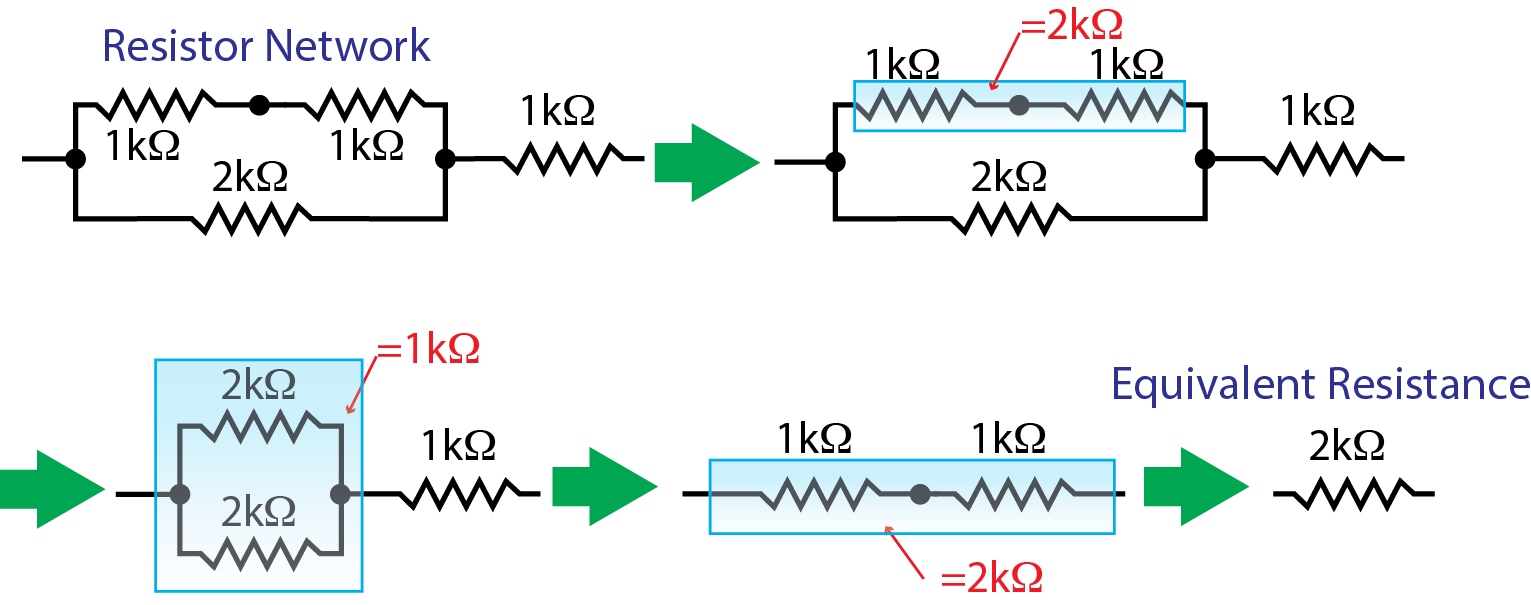
\includegraphics[width=\textwidth]{ex_resnet.png}
\end{center}
\end{figure}



%%% ========================================================================

\chapter{Circuit Analysis Fundamentals}
We will meow go on to...

\section{Elementary Circuit Analysis: An example}
\label{sec:circuitanalysis}
We can now use Ohm's law, along with the equations for parallel and series resistors to completely analyze a circuit. Not all circuits can be analyzed this way and for those, we will need a new method known as Kirchhoff's rules (section \ref{sec:kirchhoff}). 

\begin{figure}[h]
\caption{Elementary circuit analysis}
\label{fig:elemcirc}
\begin{center}
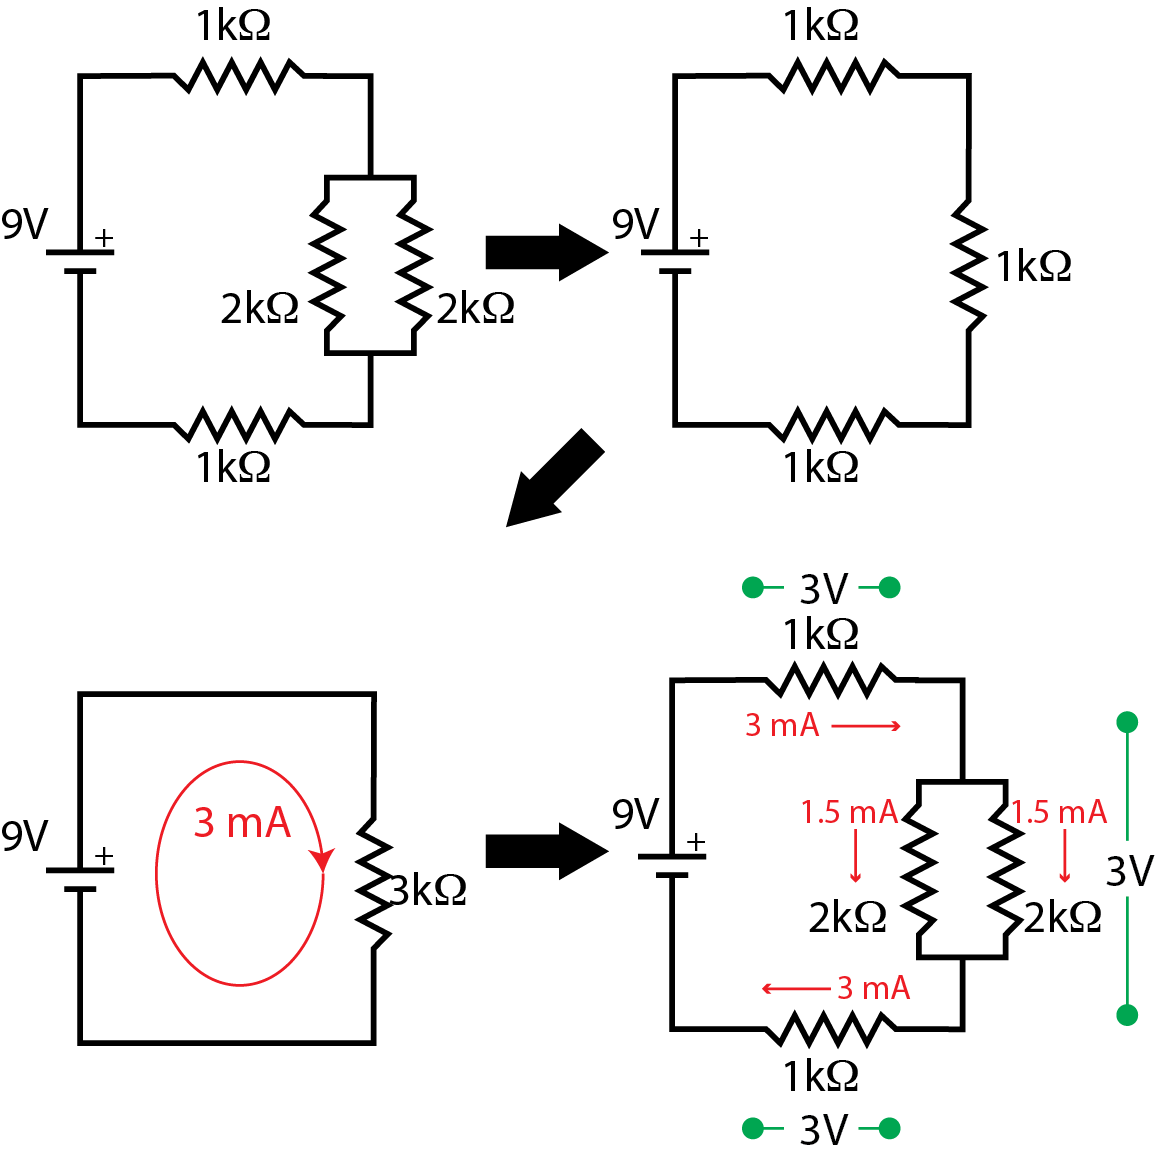
\includegraphics{elemcirc.png}
\end{center}
\end{figure}


Consider the circuit in figure \ref{fig:elemcirc}. Our goal will be to slowly fill in all the voltage drops and currents in this circuit and know all that there is to know about the circuit. First, we can reduce the parallel 2~k$\Omega$ resistors to a single 1~k$\Omega$. Next, we have 3 1~k$\Omega$ resistors in series, equivalent to a single 3~k$\Omega$ resistor. When connected to a 9~V battery, this gives a current of 3~mA. 

\noindent Now working backwards, we see the voltage drop across the parallel resistors and the two 1~k$\Omega$ resistors is $V = IR = 3~\text{mA}\times1~k\Omega = 3~\text{V}$. The current through the 2~k$\Omega$ resistors is $I=V/R = 1.5~\text{mA}$ and we know all there is to know about this circuit.
%%% ========================================================================

\chapter{Amplifiers}
\section{Active vs. Passive Circuits}
We now move into the regime of so-called \textit{active electronics}. Everything studied so far -- resistors and capacitors, to voltage dividers and filters, to diode rectifiers has fallen under the realm of passive electronics. Active electronic devices, in addition to standard inputs and outputs, require additional power supplies in order to function. There are great benefits to this, as we shall see: active components can output more power than at their input, and can eliminate annoying effects such as voltage loading due to input and output impedance. The first active device we'll study is the amplifier.
\section{The Ideal Voltage Amplifier}
The idea of the basic amplifier is simple: take the input $x_\text{in}$ and produce an output which is some number $G$ times the output.
\begin{equation}
\label{eq:simple_amp}
x_\text{out} = Gx_\text{in}
\end{equation}

\noindent ... where $G$ is known as the gain.

There is the question of what input $x_\text{in}$ is being amplified. In our course, normally $x_\text{in}$ will be a voltage and so we will have a voltage amplifier. In this case the gain is often expressed in decibels as:

\begin{equation}
\label{eq:voltage_amp_dB}
G_\text{dB} = 20\log\frac{v_\text{out}}{v_\text{in}} 
\end{equation}

We will occasionally deal with power amplifiers whose input and output is a power. For these amplifiers, the gain is also in dB but with a 10 instead of a 20 multiplier\footnote{Recall that for a fixed load resistance, $P = v^2/R \propto v^2$. Thus $10\log\left[P_\text{out}/P\text{in}\right] = 10\log\left[\left(v_\text{out}/v\text{in}\right)^2\right] = 20\log\left[v_\text{out}/v_\text{in}\right]$, thus yielding consistant definitions of gain}:

\begin{equation}
\label{eq:power_amp_dB}
G_\text{dB} = 10\log\frac{P_\text{out}}{P_\text{in}} 
\end{equation}

\noindent For now though, we will restrict outselves to voltage amplifiers. Diagrammed in figure \ref{fig:simple_amp}. The output is descibed by equation \ref{eq:simple_amp}.

\begin{marginfigure}%
  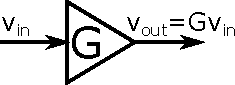
\includegraphics[width=\linewidth]{SimpleAmplifier}
  \caption{The simplest of amplifiers: the output is the input multiplied by a constant gain $G$.}
  \label{fig:simple_amp}
\end{marginfigure}

\section{Reality Check: Amplifiers in Real Life}
There are several limitations to the ideal amplifier that come into effect in practice. For example the amplifier will have to draw at least a small current from the source in order to operate. As we've learned, this is equivalent to a finite \textit{input impedance} $R_\text{in}$. The amplifier will also have a limit to how much current it can output due to its internal resistances. This leads to a finite \textit{output impedance} $R_{out}$. There are also limits to how fast the amplifier can respond to a changing input signal. This leads to a finite \textit{gain bandwidth}, or in general, a frequency dependant gain $G(\omega)$. We will examine each of these effects presently.

\subsection{Effects of Finite Input Impedance}
\label{sec:AMP_effect_input}
We can model the non-ideal amplifier as an ideal amplifier inside a black box, precisely as we did with ideal vs real voltage sources. Inside the black-box, the input impedance is models as an internal resistance $R_\text{in}$ to ground placed before the ideal amplifier. This forms a voltage divider with the input impedance from the rest of the circuit so that there is some voltage drop. The ideal amplifier thus sees a different voltage than $v_\text{in}$, which we denote $v^\prime_\text{in}$. The output of the real amplifier is thus less than we would expect: $v_\text{out} = Gv^\prime_\text{in} < Gv_\text{in}$

\begin{marginfigure}%
  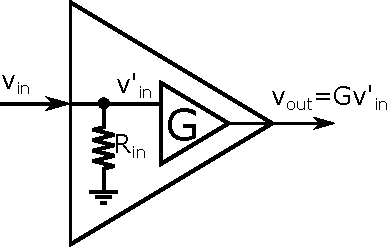
\includegraphics[width=\linewidth]{RealAmplifier_int}
  \caption{We model the finite input impedance of the amplifier as a internal resistor $R_\text{in}$ to ground before an ideal amplifier all in a black box.}
  \label{fig:real_amp_int}
\end{marginfigure}


The true output, given the input impedance can be calculated given the output impedance of whatever follows. For example, with a $100$~$\Omega$ input impedance amplifier with $G = 10$, 

\subsection{Effects of Finite Output Impedance}
The operation of our ideal amplifier can be seen as a two part process: first it senses the voltage at its input (with the effect of finite input impedance causing some loading error), and second, it acts as a new voltage source, producing a voltage $v_\text{out} Gc_\text{in}$. As with any \textit{real} source, it will be equivalent to an ideal source, in series with an output impedance $R_\text{out}$. This finite output impedance leads to a maximum short-circuit current of $v_\text{out}/R_\text{out}$ and will lead to all of the loading issues discussed in chapter XXX. Figure \ref{fig:real_amp_int_out} shows our improved model of how a real amplifier behaves.

\begin{marginfigure}%
  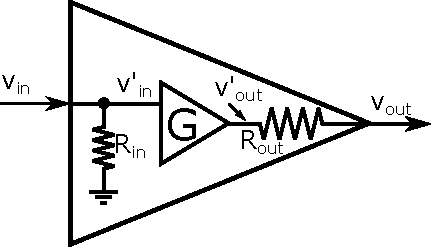
\includegraphics[width=\linewidth]{RealAmplifier_int_out}
  \caption{A better model of a real amplifier has an input resistance to ground in parallel with the inpput and an output resistance in series with its output.}
  \label{fig:real_amp_int_out}
\end{marginfigure}

\noindent\textbf{Design Example:} Consider a real amplifier with $R_\text{in} = 10$~k$\Omega$, $R_\text{F} = 100~\Omega$, and G = 25. We use it to amplify a 10~mV signal from a photodetector having $R_\text{out,PD} = 1250~\Omega$ and send it to a (lousy) voltmeter with $R_\text{in,LVM}$ = 500~$\Omega$ (see figure \ref{fig:prob_amp}). What is the voltage measured (a) assuming an ideal $G = 25$ amplifier, and (b) with our real amplifier?

\noindent Answer: For part (a) the answer is simply $v_\text{meas} = 25\times10~$mV = 250~mV. For our real amplifier, we must consider the input and output stage. The input now forms a voltage divider with $R_\text{in}$ (figure \ref{fig:prob_amp}b so that the inner ideal amplifier sees:
$$
v_\text{in}^\prime=\frac{R_\text{in}}{R_\text{out,PD} + R_\text{in}} = \frac{10~\text{k}\Omega}{11.25~\text{k}\Omega}\times10~\text{mV} \approx 8.9~\text{mV}
$$
In our model, this is then amplified by the ideal internal amplifier producing
$$
v_\text{out}^\prime = 8.9~\text{mV}\times 25 \approx 222~\text{mV}
$$
Finally, this is then sent to our lousy voltmeter, through its internal output resistance, forming another voltage divider (figure \ref{fig:prob_amp}c) to yeild the final voltage:
$$
v_\text{out} = \frac{R_\text{in,LVM}}{R_\text{out} + R_\text{in,LVM}}v_\text{out}^\prime = \frac{500~\Omega}{600~\Omega}\times 222~\text{mV}\approx 185~\text{mV}
$$

\begin{figure}[ht]
\caption{Example Problem.}
\label{fig:prob_amp}
\begin{center}
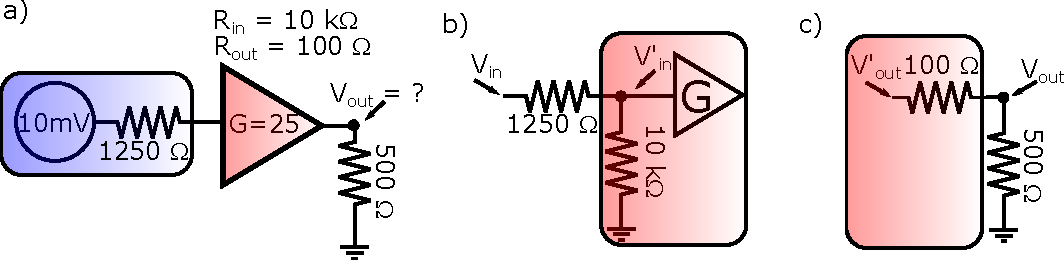
\includegraphics[width=\textwidth]{Images/amp_example.pdf}
\end{center}
\end{figure}

We thus see that the effect of finite input and output impedance is to lessen the effective gain of the real amplifier. Even if we used an ideal voltmeter with infinite input impedance, we'd still see 222~mV $<$ 250~mV. Equivalently, we could try to build an amplifier with $R_\text{out} \rightarrow 0~\Omega$ and again we'd see 222~mV, regardless of the impedance of the voltmeter. To get the full 250~mV however, we'd need to also have $R_\text{in} \rightarrow \infty$, so that $v_\text{in}^\prime = v_\text{in} = 25$~mV. 

From this we can infer the ideal characteristrics of a real amplifier: we want the input impedance as high as possible while having output impedance as low as possible. This can be accomplished using solid state transistors, discussed later in the course. 

\subsection{Effects of Noise: Noise Factor and SNR}
The ideal amplifier will amplify the voltage present at it's input, regardless of whether we consider that voltage to be useful signal or to be noise. This can lead to fundamental issues in isolating very weak signals since eventually, we will just be scaling up Johnson, Shot, or technical noise. 

For example, if you have a 10~nV signal atop 25~nV of Johnson noise, you can send your signal to a 120~dB amplifier to get 100~mV of signal, but it will still be lost in the Johnson noise, which is now at 250~mV.  We amplified the signal level, but have not improved the signal level as compared to the signal. This ratio of signal vs noise has, in a spark of linguistic creativity, been dubbed the ``signal to noise ratio'' or SNR. since the voltage of the noise is usually stochastic \footnote{ A high-brow term, effectively meaning ``random''}, usually the signal to noise ratio is usually specified in terms of power, rather than voltage\footnote{ ...wait, what $R$ should we use here? Well power is energy per unit time and that energy has to be delivered to something. That something is the load resistance, so that a given voltage noise will deliver more power to a 1$00~\Omega$ than a $100~\text{k}\Omega$ resistor} (ie. $v_{RMS}^2/R)$

\begin{equation}
\label{eq:def_snr}
\text{SNR} \equiv \frac{P_\text{sig}}{P_\text{noise}} = 10\log_{10}\left[\frac{P_\text{sig}}{P_\text{noise}}\right] \text{dB}
\end{equation}

So an amplifier on its own will not help you discern signals dominated by noise and the SNR must be improved though separate means. If your signal exits within a given range of frequencies but your noise exists at all frequencies, a filter can be applied to the input of the amplifier to greatly improve the SNR. If the  signal and noise coexist at the same range of frequencies, you have to be more clever. For example, a common source of noise is thermal motion of electrons through a load resistance. To improve the SNR, circuits are often cooled to -40 $^\circ$C or even as low as several Kelvin, when extremely faint signals are being detected.

To make matters worse, the amplifier often adds its own noise to the system - that is the SNR of the output is typically even higher than that of the input! This is quantified by the so-called noise figure:

\begin{equation}
\label{eq:def_noise_figure}
\text{NF} \equiv \frac{\text{SNR}_\text{out}}{\text{SNR}_\text{in}} = 10\log_{10}\left[\frac{\text{SNR}_\text{out}}{\text{SNR}_\text{in}}\right]
\end{equation}

\noindent Good amplifiers will have NF $2$~dB or less.

\subsection{Effects of Finite Frequency Response}
Since every circuit element has some finite capacitance and inductance, we can replace the internal input and output resistances with an input impedance $Z_\text{in}$ and output impedance $Z_\text{out}$. The net effect of this is to produce a frequency dependant gain $G(\omega)$. This can be modelled as internal frequency filter that is applied to the input or output. This bug can be rebranded as a feature as an amplifier may actually filter out high frequency noise present in the signal, as discussed in the previous section.

\section{Differential Amplifiers}
\label{sec:diff_amps}
Often in physics, it is a small deviation from a fixed value that is of interest rather than the absolute value itself. For example, a beam of light may pick up a small oscillation in intensity as compared to a reference beam when passed through a sample. In this case, a \textit{differential amplifier} may be used. As diagrammed in figure \ref{fig:differential_amplifier}, a differential amplier has two inputs and a single output corresponding to the difference between the signals. This is operation can be seen as first inverting one input and then adding it to the other. The input which is inverted $V_-$ is fitting called the ``inverting input'', while the normal input is verbosely titled the ``non-inverting input'', $V_+$. The multiplication factor is known as the ``differential gain'' $G_\text{diff}$ and is defined through the relation
\begin{equation}
\label{eq:def_diff_amp}
v_\text{out} = G_\text{diff}\left(v_+-v_-\right).
\end{equation}


\begin{marginfigure}%
  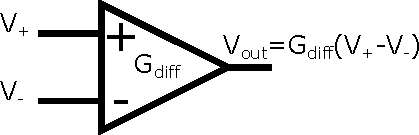
\includegraphics[width=\linewidth]{differential_amplifier}
  \caption{A Differential Amplifier.}
  \label{fig:differential_amplifier}
\end{marginfigure}


\textit{Example:} A differential amplifier with $G_\text{diff} = 40$~dB has, at its inputs: $v_+ = 3.7$~mV and $v_- = 4.2$~mV. What is the output voltage?

\textit{Solution:} The gain of 40~dB implies that $20\log_{10}\frac{v_\text{out}}{v_+-v_-} = 40$, so that $v_\text{out} = 100\left(v_+-v_-\right)$. Since, $\left(v_+-v_-\right) = \left(3.7-4.2\right)~\text{mV} = -0.5~\text{mV}$, we will find $v_\text{out} = -500~$mV.
\subsection{Common Mode Gain}
From equation \ref{eq:def_diff_amp}, we expect that if $v_+ = v_-$, we will have $v_\text{out} = 0$ regardless of the value of $v_+$ and $v_-$. In practice however, this is not the case. This can be due, for example, to differences in the input impedances of the individual inputs so that internally, $v_-^\prime \neq v_+^\prime$ even though $v_- = v_+$ (see the previous section \ref{sec:AMP_effect_input}). To quantify this, we define the \textit{common-mode voltage} as the average of the inverting vs. non-inverting input voltages:
\begin{equation}
\label{eq:common_mode_voltage}
v_\text{com} \equiv \frac{v_+-v_-}{2}
\end{equation}

The amount of signal that gets through defines the \textit{common-mode gain}
\begin{equation}
\label{eq:common_mode_gain}
v_\text{out} = G_\text{com}\frac{v_++v_-}{2}
\end{equation}
An ideal differntial amplifier would have $G_\text{com} = 0$ or $-\infty$~dB. The true output of the \textit{real} differential amplifier is thus:
\begin{equation}
\label{eq:real_diff_amp}
v_\text{out} = G_\text{diff}\left(v_+-v_-\right) + G_\text{com}\frac{v_++v_-}{2}.
\end{equation}

\subsection{Common Mode Rejection Ratio}
The ``goodness'' of a differential amplifier is how much it behaves like one! Mathematically we can quantify this by saying that for a good differential amp, $G_\text{com} \ll G_\text{diff}$. THis is represented by the so-called ``common-mode rejection ratio'' or CMRR. The CMRR is usually stated in decibels and is given by:
\begin{equation}
\label{eq:def_CMRR}
\text{CMRR} \equiv 20\log_{10}\left[\frac{G_\text{diff}}{G_\text{com}}\right]
\end{equation}
 
Decent differential amplifiers have CMRR$^\text{s}$ of at least 70~dB but some applications require 120~dB or higher.
%\subsection{Special Purpose Amplifiers}Power amplifiers, Audio Amplifiers, Instrumentation Amplifiers, oh my! Also Lock-In Amplifiers!

\chapter{Feedback and Op Amps}
By far and wide, the amplifier that you will see the most of in the labs is a very high gain, differential amplifier known as an ``operational amplifier'', or \textit{Op Amp}. Op-amps form the basis of a very wide range of applications: adding and subtracting voltages, frequency filters, low-noise single-input amplifiers, circuit protection, oscillators/fucntion generators, and analog to digital converters, (to name a few). The typical differential gain of an op-ampo is insanely high - 1,000,000 or higher. The gain is so high infact that it renders opamps useless when used as standard differential op-amps. The utility of an op-amp comes in by employing the crucial concept of negative feedback, which we will explore presently.

\section{Negative Feedback}
Feedback refers to a configuration in which the output of a system is connected back into its input (ie. ``fed back''). Feedback systems are everywhere in nature: in the human body the amount of insulin in the bloodstream is sensed and fed back into beta cells in the pancreas which determine the amount of insulin to be secreted. In climatology, a mechanism for ice ages is thought to be that colder weather creates more snow and thus more light is reflected back into space, creating more snow, etc. Of course, feedback systems can be engineered by us humans as well. The formal theory of feedback is a part of the field known as control theory.

A simple feedback system is shown in figure \ref{fig:simple_feedback}a.

\begin{figure}[ht]
\caption{a) The simplest feedback system. b) Opamp in negative feedback configuration. If the output was wired to the non-inverting input, it would be ``positive feedback''.}
\label{fig:simple_feedback}
\begin{center}
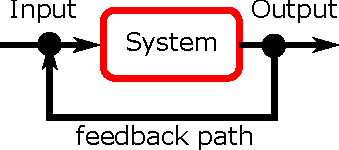
\includegraphics[]{Images/simple_feedback.pdf}
\end{center}
\end{figure}

\section{Op Amps in Negative Feedback: The Golden Rules}
Let's observe the operating characteristics of an ideal opamp, operating in a simple negative feedback configuration as diagrammed in figure \ref{fig:simple_feedback}b. We can look at both in terms of an abstract feedback system and also try to get a picture of what's going on ``under the hood''. Let's start with the former: We don't know what the output actually is, but from the definition of a differential amplifier (equation \ref{eq:def_diff_amp}), and from the fact that the output is wired to the the inverting input (hence negative feedback) we see that $v_+ = v_\text{in}$ and $v_-=\text{out}$. Thus:

\begin{equation*}
v_\text{out} \equiv G\left(v_+ - v_-\right)  = Gv_\text{in} - Gv_\text{out}
\end{equation*}

\noindent ... so that 
\begin{equation}
\label{eq:opamp_analysis_feedback}
v_\text{out} = \left(\frac{G}{G-1}\right)v_\text{in}
\end{equation}
In the limit of an ideal opamp, $G\rightarrow\infty$ so that this becomes $v_\text{out} = v_\text{in}$. Congratulations, we've just made the worlds most useless circuit. Or have we? In fact, although I chose this as a simple way to understand opamps, this circuit, known as a ``buffer op-amp'' is indeed very usefull and is found everywhere. Why? Because of the other property of the opamp - the insanely high input impedance. This means that the non-inverting opamp ``sniffs-out'' the input voltage while drawing negligable current, reproducing the voltage at the output and providing whatever current is called for. But where does this current come from if not the input? It turns out that we forgot to draw all of the opamp's terminals on our sketch - op-amps are active components and thus need power. Whatever power is needed for the output essentially comes from the power terminals and our buffer opamp thus separates whatever is on the input side of the circuit from the components on the output. We can drive large amounts of current without disturbing the sensor, voltage divider, or whatever is going into the circuit. No loading error, near zero output impedance. The buffer opamp creates a signal and converts it into a near-ideal source.

The above example illustrates the most important features of opamps in negative feedback. They are so useful in understanding how opamps behave, that they have been dubbed ``The Golden Rules of OpAmps'':

\textbf{Golden Rule I}: The opamp draws no current at its inputs: $i_+ = i_- = 0$.

\textbf{Golden Rule II}: In negative feedback, the opamp's output adjusts itself so that it' inputs are equal $v_+ = v_-$.

The first rule is merely a restatment that opamps have very large input impedance. The second rule is a property of negative feedback, but is less obvious than the first. To understand why it must be so, lets reanalyze the previous example in a more empirical manner. Consider again the circuit in figure \ref{fig:simple_feedback}b. Suppose we have just switched the circuit on and the output is some random value (I don't know ... $-1.234$~V say) and the input is at 3~V. The input sees a voltage diference of 4.234~V and immediately starts trying to put out an enormous, positive voltage (although it can't sitch instantaneously, since there's always some capacitance inductance and resistance in the circuit.) Thus a split secon later, the output difference has been reduced, say to +2V. Now the output difference is 1~V and again the output tries to become more positive (but less than before.) After a short time the output reaches +3~V and the output no longer tries to swing to a more positive value. Suppose that it overshoots 3~V (due to its small parasitic inductance) so that the voltage is now at 3.1~V. The difference voltage is now -0.1~V and the output now starts becoming negative. We see the action of negative feedback on the system -- when the output is lower than the input it quickly becomes larger and when it is higher, it quickly becomes lower. The only stable configuration is where the output equals the input. This is why \textbf{GR II} works. 

\begin{marginfigure}%
  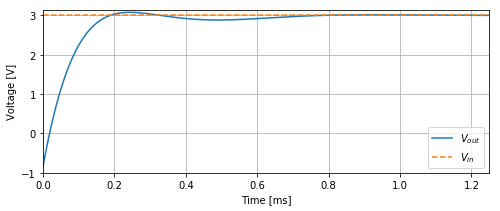
\includegraphics[width=\linewidth]{feedback_time_dep}
  \caption{Feedback quickly settles the output value to whatever the input happens to be.}
  \label{fig:feedback_time_dep}
\end{marginfigure}

Of course, we can do much more with opamps than to create a voltage buffer. There are, quite literally, shelves in libraries filled with entire books on opamps. We'll go through the more common opamp applications in the following sections. We can use the golden rules of opamps throughout to analyze the functionality of these circuits.

\subsection{Inverting Opamps}
The next simplest opamp to analyze is the inverting opamp, seen in figure \ref{fig:inv_noninv_opamps}a. Here the gain is a negative number so that a positive input produced a negative output and vice versa. 

To understand the functionality of this opamp, we apply the golden rules. First, since the non-inverting output is shorted to ground \textbf{GR II} tells us that the noninverting terminal is also clamped to ground. In this situation, the node at the inverting terminal is said to be a \textit{virtual ground}. The current through the first resistor $R_1$ is thus:

\begin{equation}
\label{eq:inverting_opamp_deriv_1}
i_{R_1} = \frac{v_+}{R_1}
\end{equation}

Next, \textbf{GR I} tells us that no current runs into the $v_+$ terminal so that by Kirchhoff's rules, $i_{R_2} = i_{R_1} = v_+/R_1$. This allows us to determin the voltage drop across the second resistor $R_2$ (note now that the voltage goes from 0 to something lower):
\begin{equation}
\label{eq:inverting_opamp_deriv_2}
0-v_\text{out} = i_{R_2}R_2 = \frac{R_2}{R_1}v_+
\end{equation}

This gives us the output of the inverting opamp:

\begin{equation}
\label{eq:inverting_opamp}
v_\text{out} = -\left(\frac{R_2}{R_1}\right)v_+
\end{equation}

The gain is negative and adjustable by adjusting $R_1$ or $R_2$.

\begin{figure}[ht]
\caption{a) Inverting opamp with gain $G=-R_2/R1$. b) Non-inverting opamp with gain $G = 1+R_2/R_1$}
\label{fig:inv_noninv_opamps}
	\begin{center}
		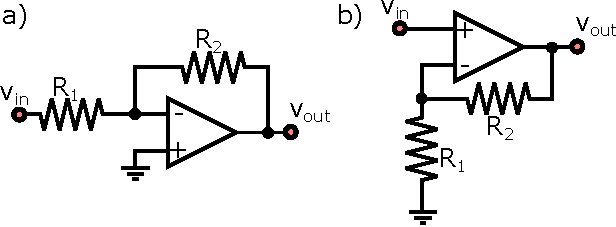
\includegraphics[]{Images/inv_noninv_opamps.pdf}
	\end{center}
\end{figure}


\subsection{Non-Inverting Opamps}
The next opamp that we will analyze is the ``non-inverting'' opamp of figure \ref{fig:inv_noninv_opamps}b. Here we can use the second golden rule to note that the inverting terminal is held at whatever $v_\text{in}$ is. In order to determine the output voltage, we note again that \textbf{GR I} tells us that no current runs into the $v_-$ terminal and so that $R_1$ and $R_2$ form a voltage divider from $v_\text{out}$ to ground with $v_- = v_\text{in}$ as the intermediate voltage:

\begin{equation}
\label{eq:noninverting_opamp_deriv_1}
v_\text{in} = \frac{R_1}{R_1 + R_2}v_\text{out}
\end{equation}

Rearranging to solve for $v_\text{out}$, we find: 

\begin{equation}
\label{eq:noninverting_opamp}
v_\text{out} = \left(1+\frac{R_2}{R_1}\right)v_\text{in}
\end{equation}
Although the noninverting output has the benefit of a positive gain, a limitation is that unlike its inverting counterpart, it can not have $\vert G\vert < 1$.

\subsection{Differential Amplifiers}
Although the ultra-high gain of an opamp makes it fairly useless as a direct differential amplifier, we can make a differential amplifier circuit using an opamp. The use of feedback can ensure low output impedance, tuneable differential gain, and high CMRR (see section \ref{sec:diff_amps}).

The opamp-based differential amplifier is shown in figure [zzz]. Pairs of matched resistors $\left(R_1,R_2\right)$ are used for the feedback path. As usual, we can derive the output in terms of the golden rules: \textbf{GR I} tells us that the top and bottom paths form voltage dividers between $v_1\rightarrow v_\text{out}$ and $v_2\rightarrow \text{GND}$ respectively, ie.

\begin{align*}
\frac{v_--v_\text{out}}{v_1-v_\text{out}} &= \frac{R_2}{R_1+R_2} \\
\frac{v_+-0}{v_2-0} &= \frac{R_2}{R_1+R_2} 
\end{align*}

\noindent ... rearranging, we find:

\begin{align}
v_- &= \frac{R_1v_\text{out} + R_2v_1}{R_1+R_2} \\
v_+ &= \frac{R_2}{R_1+R_2}v_2
\end{align}



From \textbf{GR II} we know that these inputs are equal. Equating them and multiplying both sides by $R_1 + R_2$, we find $R_2v_2 = R_1v_\text{out} + R_2v_2$, or

\begin{equation}
\label{eq:differential_opamp}
v_\text{out} = \frac{R_2}{R_1}\left(v_2-v_1\right)
\end{equation}

We thus have a differential amplifier with adjustible gain ($R_2/R_1$). There are two issues with this design however. First, it requires perfectly matched resistors or else the output will not be directly proportional to the voltage difference. Next, small differences in the input stages of real opamps lead to imperfect cancellation of common mode signals. For this reason, some opamps provide extra ``offset-null'' pins which can be used to compensate for these differences. In the lab you will build your own differential opamp and do just this.

\subsection{Differentiator and Integrator Opamps}
We now consider the effect of general impedances in the construction of opamp feedback circuits. Fortunately, out generalized Ohm's law analysis that we analyzed earlier allows us to quickly determine the gain of the circuit, which when using reactive components is generally frequency dependant. 

\subsection{Differentiator Circuit}
Consider first, the circuit in figure \ref{fig:differentiator_opamp}a. \textbf{GR I} tells us that the current throught the capacitor is equal to that of the resistor $i_C = i_R \equiv \left(v_--v_\text{out}\right)/R$, while \textbf{GR II} tells us that $v_-$ is a virtual ground ($v_- = 0$). Recalling the definition of a capacitor:

\begin{equation}
\label{eq:defn_capacitor_rep}
i_C = C\frac{dv_C}{dt}
\end{equation}

we have, noting $v_C = v_\text{in}$:

\begin{equation}
\label{eq:opamp_differentiator}
v_\text{out} = -RC\frac{dv_\text{in}}{dt}
\end{equation}
\noindent ... ie. the output is the derivative of the input voltage, scaled by a factor of $-RC$.

\begin{figure}[ht]
\caption{a) Differentiator opamp: $v_\text{out} = -RCv_\text{in}^\prime(t)$. b) The addition of a ``roll-off'' capacitor fixes the differentiator's susceptibility to high frequency noise.}
\label{fig:differentiator_opamp}
	\begin{center}
		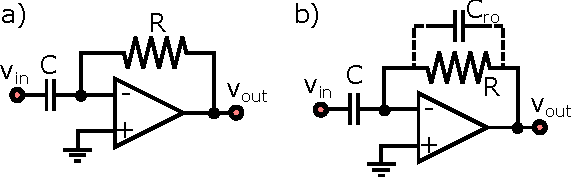
\includegraphics[]{Images/differentiator_opamp.pdf}
	\end{center}
\end{figure}
\subsection{A better Differentiator Circuit}
A problem with derivatives is that very fast signals will produce enourmous outputs. Even small amounts of noise can be greatly amplified, for a Fourier component at frequency $\omega$, given by $v_\omega(t) = v_0e^{j\omega t}$ has a derivative with magnitude:

$$
\left\vert\frac{dv_\omega(t)}{dt}\right\vert = \omega \vert v_\omega(t)\vert
$$

Thus a $1~\mu$V signal at 10~MHz will have an amplitude of over 30~V! A stadard trick to overcome this is to put a small, roll-off capacitor $C_\text{ro}$ in parallel with the feedback resistor (figure \ref{fig:differentiator_opamp}b). At lower frequecies ($\omega \ll 1/RC_\text{ro}$) the extra capacitor has very high resistance and the feedback current is completely dominated by the resistor ($Z_2 \approx R$). The situation is identical to the previous analysis. For very high frequencies however, the capacitance now has vanishing impedance and the current would rather ignore the resistor and take this path ($Z_2\approx -j/\omega C_\text{ro}$) and the gain rolls off to zero at high frequencies.

\subsection{Integrator Circuit}
A slight modification to the differentiator circuit is shown in figure \ref{fig:integrator_opamp}a. Here the non-inverting input is still held at a virtual ground but the positions of the resistor and capacitor are swapped. Now, we have
$$
i_C = -C\frac{dv_\text{out}}{dt} = \frac{v_\text{in}}{R}
$$

Integrating this equation gives
\begin{equation}
\label{eq:opamp_integrator}
v_\text{out}(t) = -\frac{1}{RC}\int_{t_0}^{t}v_\text{in}(t)dt =  -\frac{1}{RC}\int v_\text{in}dt + k_0
\end{equation}

\noindent so that we have an output that is the integral of the input. The constant of integration is given by the value of the input at $t_0$, ie. $k_0 = -\frac{v_\text{in}(t_0)}{RC}$.

\begin{figure}[ht]
\caption{a) Integrator opamp: $v_\text{out} = -\frac{1}{RC}\int v_\text{in}(t)dt$. b) The addition of an ``anti-windup'' resistor prevents a DC bias from overwhelming the signal. c) Alternatively, a ``reset switch'' can reset the initial condition to 0~V.}
\label{fig:integrator_opamp}
	\begin{center}
		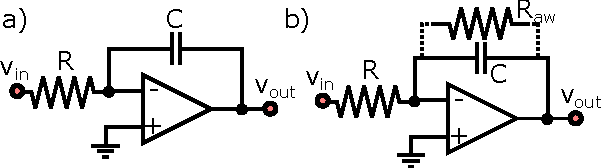
\includegraphics[width = \textwidth]{Images/integrator_opamp.pdf}
	\end{center}
\end{figure}

\subsection{A Better Integrator Circuit}
Much like the differentiator, the intrgator circuit experiences its own drawbacks. The primary is that of ``wind-up''. Wind-up is merely a statement that the integral of a constant is a constantly increasing (or decreasing) signal. Suppose that your signal is 0~V to 1~V sine wave at frequency $\omega = 2\pi\times5$~Hz and is input to an $R =  5~\text{k}\Omega$, $C = 10~\mu F$ integrator. You might expect that the output will be:

$$
v_\text{out} = -\frac{1}{RC}\int\sin(\omega t)dt = \frac{1000~\text{s}^{-1}}{\omega}\cos(\omega t) \approx 0.637~V\cos(2\pi\times5~\text{Hz})
$$

\noindent but instead, will find strange behaviour. Figure \ref{fig:windup_error} displays the resulant output when an opamp with $\pm3.3$~V supply rails are used. The output gradually drifts downward until eventually becoming a constant -3.3~V. What went wrong? Well our 0-1~V sine wave is really not a pure sine wave but a 0.5~V amplitude sine wave plus a 0.5~V constant offset. The output is then:

$$
v_\text{out} = -\frac{1}{RC}\int0.5\left(\sin(\omega t) + 1\right)dt \approx 0.637~V\left(\cos(\omega t) - t\right)
$$

\noindent ... ie. a cosine wave with a constantly decreasing offset which eventually exceeds the supply rails. This is an example of windup. There are two basic ways of resolving the issue. One way is to use a feedback resistor in parallel with the capacitor (figure \ref{fig:integrator_opamp}b), so that at very low frequencies (and at DC) the near-infinite impedance of the capacitance is bypassed by the ``anti-windup'' resistor, capping the gain at $-R_\text{aw}/R$. A second way is to place a manual or automatically activated switch in place of $R_\text{aw}$ (figure \ref{fig:integrator_opamp}c) which shorts the gain to zero. THis can be seen as setting the initial condition to zero.

\begin{marginfigure}%
  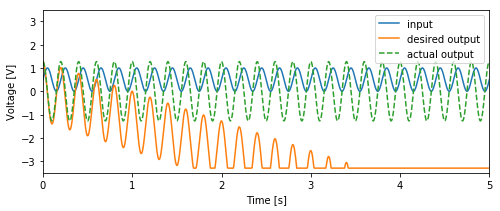
\includegraphics[width=\linewidth]{windup_error}
  \caption{Windup error.}
  \label{fig:windup_error}
\end{marginfigure}


\backmatter

% \bibliography{sample-handout}
% \bibliographystyle{plainnat}


\printindex

\end{document}
